% !TEX encoding = UTF-8 Unicode
\documentclass[a4paper]{article}

\usepackage{graphicx}
\usepackage[english,serbianc]{babel}
\usepackage[unicode]{hyperref}
\hypersetup{colorlinks,
                   citecolor=green,
                   filecolor=green,
                   linkcolor=blue,
                   urlcolor=blue}

% Овако фонт неће бити блед тј. инсталираће
% се квалитетни фонтови за случај да већ нису
\usepackage{type1ec}

% Овако је могуће претраживати и копирати ћирилицу
% из генерисаног документа, независно од хифенације
\usepackage{cmap}
\defaulthyphenchar=127

% Овако је могуће у табели имати текст у два реда
\newcommand{\dvareda}[2][c]{\begin{tabular}[#1]{@{}c@{}}#2\end{tabular}}

% Овако је могуће табеларно представити ауторе
\newcommand{\autori}[4]{\author{\begin{tabular}{c c} \dvareda{#1\\\normalsize{#2}} & \dvareda{#3\\\normalsize{#4}}\medskip \end{tabular}}}

% Овако је могуће избећи испадање алгоритма из маргина
\usepackage[linesnumbered,ruled]{algorithm2e}
\newenvironment{algoritam}[1][htb]
{\renewcommand{\algorithmcfname}{Алгоритам}
\begin{figure}[ht]
\centering
  \begin{minipage}{.75\linewidth}
	\begin{algorithm}[#1]%
  }{\end{algorithm}
  \end{minipage}
\end{figure}}

% Овако је могуће имати кључне речи
\providecommand{\keywords}[1]
{
	\small	
	\textbf{\textit{Кључне речи ---}} #1
}

\begin{document}

\title{Трансформација петљи помоћу Кланга\\ \small{Семинарски рад у оквиру курса\\Конструкција компилатора\\Математички факултет, Београд}}

\autori{Лазар Васовић}{mi16099@alas.math.rs}{Јелена Јеремић}{mi16062@alas.math.rs}

\date{23. јун 2020.}

\maketitle

\abstract{Размотрена је употреба Кланга као библиотеке у циљу трансформације свих петљи у \textit{C} коду у жељени тип (\textit{for}, \textit{while}, \textit{do-while}). На основу уводних разматрања имплементирана је апликација, у које сврхе је коришћен Клангов апликативни програмски интерфејс према апстрактном синтаксном стаблу. Саме измене вршене су у тексту кода. Описано је неколико изазова и проблема -- како успут решених, тако и отворених -- а неки су илустровани пратећим (тест) примерима.}

\keywords{Кланг (\textit{Clang}), \textit{AST}, језик \textit{C}, петље}

\tableofcontents

\newpage

\section{Увод}

Кланг (\textit{Clang}) представља предњи део компилатора, са задатком анализе и превођења \textit{C}-оликих језика \cite{clang}. Један је од основних потпројеката преводилачке инфраструктуре \textit{LLVM}, па се често спојено назива \textit{Clang/LLVM}. Осим што се може користити као алат за превођење \textit{C/C++/Objective-C} кода на међурепрезентацију, могуће је употребити га и као библиотеку, по чему се издваја међу конкурентима. Та особина следи из чињенице да пружа чист апликативни програмски интерфејс (\textit{API}), тако да га је без проблема могуће у коду користити у другим пројектима. У овом раду је истражен Клангов \textit{API} према апстрактном синтаксном стаблу (\textit{AST}) на примеру језика \textit{C}, и то конкретно на примеру трансформације петљи у жељени тип.

Петље су један од главних конструката виших императивних језика, настао са развојем структурне (пот)парадигме \cite{kozen}. Њима је уведено понављање (итерација) као нови вид контроле тока извршавања програма. Данас су неизбежан елемент већине процедуралних језика вишег нивоа, па и нешто старијег језика \textit{C}, који је овде размотрен. У њему постоје три типа петљи: \textit{for}, \textit{while}, \textit{do-while} (\textit{do}). Како је конкретан решавани проблем промена петљи из једног типа у други, постоји шест трансформација које су имплементиране. Детаљније информације о примењеном шаблону измена изложене су у телу рада.

Што се тиче самих \textit{C}-овских петљи, главне компоненте сваке јесу услов (један израз типа који се може претворити у целобројни) и тело (једна наредба, али може бити и сложена). Тако се нпр. \textit{for} и \textit{while} извршавају тако што им се прво израчунава услов, а затим и тело уколико је услов испуњен (добијена је целобројна ненула вредност), и тако укруг, све док је услов испуњен или се на неки други начин не искочи из петље. Опционо, \textit{for} омогућава да се пре прве итерације изврши иницијализација (једна наредба), а на крају сваке инкрементација (корак петље, исто једна наредба). Тип \textit{do-while} по свему личи на \textit{while}, осим по томе што му се у првој итерацији тело изврши без евалуације услова. Петље дозвољавају и два додатна механизма контроле тока унутар тела -- наредбе \textit{break} и \textit{continue}. Прва искаче из петље, преусмеравајући контролу на излаз из ње, док друга прескаче текућу итерацију, преусмеравајући контролу на крај тела петље.

\section{Апликација}

У складу са уводним разматрањима проблема, написана је апликација која трансформише петље по корисниковој жељи. Пре превођења (билдовања) програма неопходно је инсталирати шесту верзију \textit{LLVM}-а (\textit{llvm-6.0-dev}) и Кланга (\textit{libclang-6.0-dev}) за развијаоце апликација, као и алат за лепо форматирање кода (\textit{clang-format}). Приложена датотека за аутоматску изградњу извршиве верзије заснована је на систему \textit{CMake}, а за сам процес предложен је \textit{build} директоријум.

Како је већ напоменуто, три петље са могућношћу промене сваког типа у сваки други дају укупно шест могућих трансформација. Главни изазов тог посла јесте одржавање што веће семантичке (значењске) једнакости са петљом пре транформације. У овиру рада је заправо имплементирано пет трансформација, пошто је једна извршена посредно -- зарад лакшег очувања семантике контроле тока, код промене \textit{do} у \textit{while} прво је свако \textit{do} претворено у \textit{for}, па тек онда свако \textit{for} у \textit{while}. Имплементирана је и помоћна трансформација која припрема \textit{for} петље за даљи рад. Целокупан ток дат је алгоритмом \ref{alg}. Свака трансформација заснована је на особинама полазне и циљне петље, а имплементирана је прослеђивањем парсеру стабла посебно направљених класа које наслеђују Клангове класе \textit{ASTConsumer} и \textit{RecursiveASTVisitor}, редом задужене за обраду (конзумацију) и рекурзивни обилазак (посету) апстрактног синтаксног стабла. Одговарајуће текстуалне измене кода врши преписивачка класа \textit{Rewriter}.

\begin{algoritam}[H]
\SetAlgoLined
\DontPrintSemicolon
\uIf{промена на do}
     {замени свако \textit{while} са \textit{do}}
\Else{замени свако \textit{do} са \textit{for}}
\;
\uIf{промена на for}
     {замени свако \textit{while} са \textit{for}}
\Else{припреми свако \textit{for}}
\;
\uIf{промена на while}
     {замени свако \textit{for} са \textit{while}}
\uElseIf{промена на do}
            {замени свако \textit{for} са \textit{do}}
\caption{Трансформација петљи}
\label{alg}
\end{algoritam}

Идући редом, прва конкретна трансформација јесте замена сваког \textit{while} са \textit{do} (линија 2). Ово је одрађено релативно простим преусмеравањем аргумената полазне петље на циљну, уз додатак испитивања услова пре прве иначе безусловне итерације циљне петље. Примењени шаблон измене дат је сликом \ref{while2do}, са разматраном \textit{C}-овском синтаксом.

\begin{figure}[h!]
\begin{center}
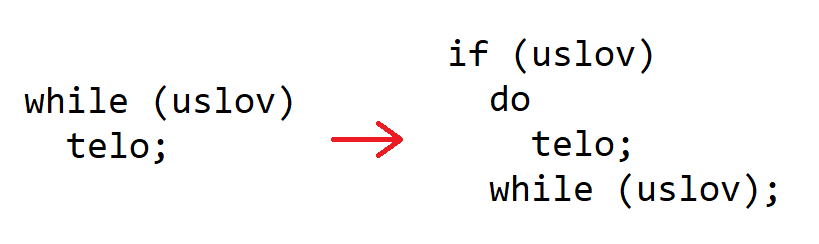
\includegraphics[scale=0.6]{while2do.png}
\end{center}
\caption{Замена сваког \textit{while} са \textit{do}}
\label{while2do}
\end{figure}

Следећа је замена сваког \textit{do} са \textit{for} (линија 4). Ово је најкомплекснија трансформација, која укључује увођење помоћне променљиве за складиштење евалуираниог услова. На почетку, он је тривијално испуњен, тако да је варијаблина почетна вредност целобројна јединица, док се за корак петље узима израчунавање услова и његова додела. Иницијализација је празна. Схема трансформације дата је сликом \ref{do2for}.

\begin{figure}[h!]
\begin{center}
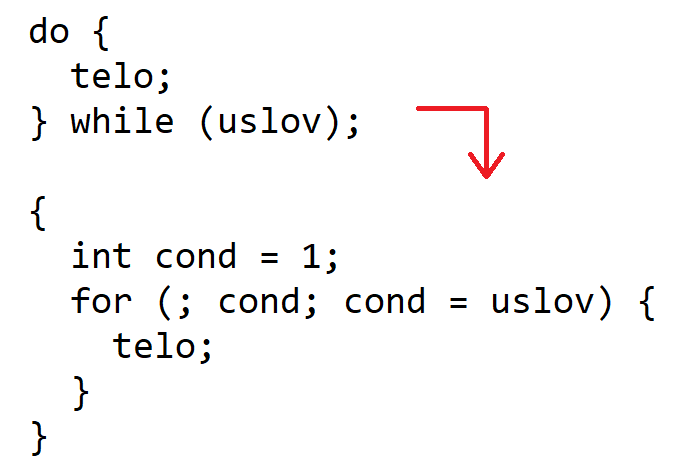
\includegraphics[scale=0.6]{do2for}
\end{center}
\caption{Замена сваког \textit{do} са \textit{for}}
\label{do2for}
\end{figure}

Наредна је замена сваког \textit{while} са \textit{for} (линија 8). Ово је најтривијалнија трансформација, пошто подразумева само преусмеравање тела и услова, док иницијализација и корак циљне петље остају празни. Шаблон ове измене илустрован је сликом \ref{while2for}.

\begin{figure}[h!]
\begin{center}
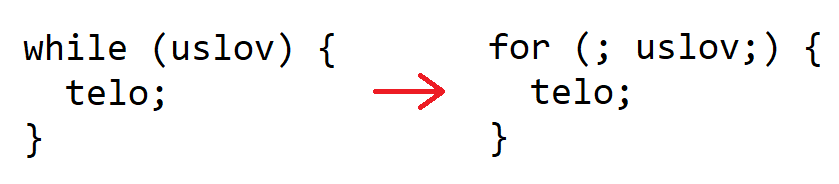
\includegraphics[scale=0.6]{while2for}
\end{center}
\caption{Замена сваког \textit{while} са \textit{for}}
\label{while2for}
\end{figure}

Разлог припреме \textit{for} петљи пре даљег рада (линија 10) изложен је у поглављу посвећеном проблемима. Засад је довољно напоменути да је ово урађено тако што је испред сваког \textit{continue} чији је први предак \textit{for} додат корак петље, наравно, уколико петља уопште има корак.

Следи замена сваког \textit{for} са \textit{while} (линија 14). Ова трансформација своди се на преусмеравање тела и услова, уз додатак да се пре циљне петље мора извршити иницијализација полазне, уколико она постоји, док се на крају тела циљне петље евалуира корак полазне, опет уколико постоји. Схема примењене измене дата је сликом \ref{for2while}.

\begin{figure}[h!]
\begin{center}
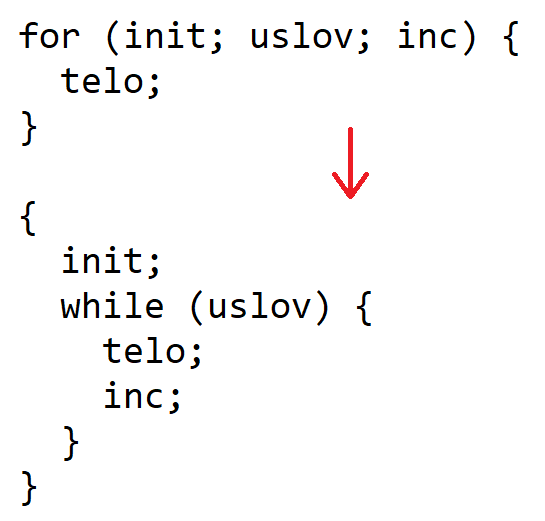
\includegraphics[scale=0.6]{for2while}
\end{center}
\caption{Замена сваког \textit{for} са \textit{while}}
\label{for2while}
\end{figure}

Напослетку преостаје замена сваког \textit{for} са \textit{do} (линија 16). Она је идентична композицији замене \textit{for} са \textit{while}, а затим \textit{while} са \textit{do}, али је засебно имплементирана зарад бољих перформанси (један пролаз уместо два) и бољег уклапања у изложени општи алгоритам. Због те еквивалентности, ипак, за њу није приложена илустрација.

Апликација као аргументе командне линије прима улазну и излазну дадотеку, као и жељени тип петље, који учествује у условима алгоритма. Приликом сваке описане трансформације изнова се формира и обрађује \textit{AST}, док се текстуалне измене кода инкрементално очитавају у излазној датотеци. На крају се лепо форматира нови код, пошто се приликом измена не брине о конзистентном увлачењу линија.

\section{Проблеми}

Упркос великој робусности Кланговог \textit{AST}-а и ширини интерфејса према њему, постоји неколико проблема на које се наишло приликом рада. Неки су настали због ограничења самог \textit{API}-ја, а неки су општи изазови који неминовно следе из рада са (\textit{C}-овским) петљама, односно из посебности њихове семантике. Неки су успешно решени, неки нису, али су сви издвојени и објашњени, неки уз пратеће (тест) примере.

Један од главних јесте имутабилност (непроменљивост) генерисаног \textit{AST}-а, као ограничење \textit{API}-ја. Наиме, чворове Кланговог синтаксног стабла није могуће мењати нити превезивати. Један од разлога за то је чињеница да Кланг не испоручује сирово стабло генерисано у току синтаксне анализе, већ успут врши и семантичку анализу, те генерише цео тзв. \textit{AST} контекст, попуњен подацима о парсираном програму. Анотирано стабло, сем нпр. информација о типовима, садржи и ситне детаље попут линије и индекса почетног и крајњег карактера у коду где је оно што чвор представља реализовано. Овакви подаци би ручном манипулацијом изгубили смисао, те би било неопходно још једном испитати значење. Директна последица овога је да није могуће лако манипулисати угнежђеним петљама. У идеалном случају, било би могуће изменити прво унутрашњу петљу, па одмах затим спољашњу, у једном пролазу нагоре, или обрнуто у једном пролазу надоле. Ипак, како измена стабла није дозвољена, а чворови не виде текстуалне измене, то овде није могуће, али је решено увођењем вишепролазности. Функција обраде заправо је бесконачна петља која у једном пролазу обради само највише спољашње чворове и не иде дубље. Она се прекида када више нема измена, а гаранцију заустављања пружа чињеница да се хијерархија угнежђених петљи у свакој итерацији смањује. Аналоган проблем је код припреме \textit{for} петљи.

Следећи важан проблем јесте контрола тока специфична за петље. Како је већ наведено, у питању су наредбе \textit{break} и \textit{continue}, од којих прва искаче из петље, преусмеравајући контролу на излаз из ње, док друга прескаче текућу итерацију, преусмеравајући контролу на крај тела петље. Оне су један од разлога зашто неколико наивних идеја за трансформације -- нпр. она према којој је \textit{do} петљу могуће претворити у друге тако што се тело избаци испред петље -- није прихватљиво решење. Ипак, уколико тело приликом сваке измене остаје на свом месту, онда \textit{break} не представља проблем, јер на исти начин искаче из петље независно од њеног типа. С друге стране, \textit{continue} има проширено значење у случају \textit{for} петљи, пошто пре преласка на следећу итерацију изврши корак петље, уколико он постоји. Прецизније, значење је и даље исто -- преусмерење контроле на крај тела петље -- али је додатак што се иза тела налази корак петље пре скока на почетак и проверу услова. Ипак, како ова финеса није видљива преко \textit{C}-овског интерфејса, у раду се сматра да је значење проширено. Проблем неједнаког значења \textit{continue} у \textit{for} и осталим типовима решен је реализацијом припремног корака који испред сваког \textit{continue} чији је први предак \textit{for} додаје корак петље, наравно, уколико петља уопште има корак. Ово можда није најбоље решење, пошто након овог корака ниједна нетрансформисана \textit{for} петља није једнака изворној, али се највише уклапа у претходно разматрану вишепролазност и не представља проблем уколико апликација успешно заврши са радом.

Пример ситног проблема са \textit{API}-јем јесте то што се празна иницијализација или корак код \textit{for} петљи не сматрају празним (нултим) наредбама, већ недостајућим вредностима, па је неопходно пазити на нулте показиваче (\textit{nullptr}). Ово се, додуше, може схватити и као предност, пошто омогућава да нпр. прелазак са \textit{for} на \textit{while} не буде компликован као на слици \ref{for2while}, већ врло једноставан, као инверз слике \ref{while2for}. Ово упрошћавање је и примењено, што се може видети по тест примерима. Када је у питању упрошћавање, могло би се помислити и да је трансформацију \textit{do} у \textit{for} са слике \ref{do2for} лако сажети убацивањем декларације са иницијализацијом условне променљиве у део за иницијализацију петље. То у неку руку јесте истина, али овде наменски није урађено, јер резултујући програм не би био у складу са \textit{ANSI C} стандардом, који многи програми прате, па би таквом изменом били покварени.

Један ситан семантички проблем који је успешно решен јесте проблем досега иницијализационе променљиве у \textit{for} петљама. Иако се при решавању претходно описаног проблема пазило да све лепо ради са \textit{ANSI C} стандардом, подржани су и \textit{C99} и новији као улаз, тако да је било неопходно обрадити и тај случај, када је пример обрнут. Наиме, иницијализациона променљива има досег који је у хијерархији између блоковског досега саме петље и досега блока изван петље. Да је нпр. при трансформацији \textit{for} у \textit{while} са слике \ref{for2while} иницијализација просто стављена испред петље, без обазирања на околину, нашла би се у спољашњем досегу. Тиме би потенцијално изазвала конфликт са већ постојећим објектом истог имена. Из тог разлога је направљен нови блок који обухвата иницијализацију и петљу, чиме се одржава полазна семантика, иако на први поглед можда не изгледа смислено.

Нешто већи проблем са досегом праве \textit{for} петље које у телу маскирају (енгл. \textit{shadowing}) имена која се користе у кораку. Наиме, у том случају простом припремом у виду додавања корака испред сваког \textit{continue} не постиже се жељени ефекат. Ово, међутим, није могуће решити локално, јер замаскирана имена у језику \textit{C} није могуће одмаскирати. Пример решења јесте одустајање од претходно објашњене апроксимације да \textit{continue} има проширено значење у случају \textit{for} петљи и прихватање чињенице да је увек у питању преусмерење контроле на крај тела петље. Тако би се нпр. за претварање \textit{for} у \textit{while} уместо схеме са слике \ref{for2while} могао користити шаблон са слике \ref{for2while2}. То ипак у овом раду није урађено, пошто се безусловним скоковима спушта на ниво непримерен структурном програмирању, чијег су петље основица.

\begin{figure}[h!]
\begin{center}
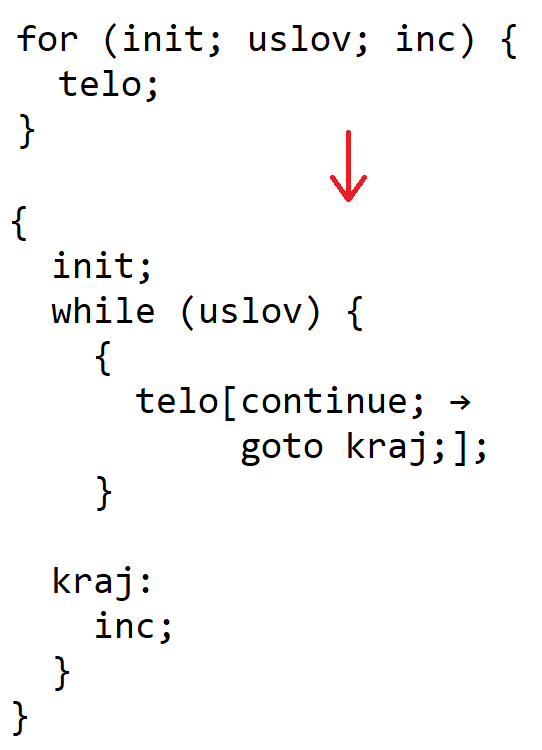
\includegraphics[scale=0.57]{for2while2}
\end{center}
\caption{Замена сваког \textit{for} са \textit{while}}
\label{for2while2}
\end{figure}

Сличан овоме је проблем са именима при увођењу помоћне условне променљиве, као на слици \ref{do2for}, при чему је неопходно пазити да се не узме неко већ заузето име, било да је глобално или важно локално. Због ограничења \textit{API}-ја ово није могуће решити без измена изворног кода Кланга, што је заправо легитиман начин рада са \textit{LLVM}-ом, али му се ипак није прибегло. Испољавање оба проблема приказано је у прикладно названом тест примеру, у пратећем \textit{test} директоријуму.

Напослетку, једини примећен нерешени проблем, тачније скуп проблема који нису решени, чине све грешке које настају при раду са претпроцесором. Наиме, језик \textit{C} има веома развијену и често коришћену инфраструктуру која претходи самом процесу превођења. Мада је основна улога претпроцесирања укључивање декларација из заглавља, распрострањена је употреба макроа и великог броја других претпроцесорских директива. Постоји и велики број условних директива, као и неких које значајно утичу на даљи процес превођења (нпр. прагме), чиме претпроцесор подсећа на преводилац у малом. Предњи део компилатора види само резултате претпроцесирања, тако да није лако реконструисати шта је тачно било у изворном коду. За ову проблематику нису формирани тест примери, али је илустрација дата кроз слику \ref{pretproc}. Са ње се види да један исечак кода може дати два резултата након претпроцесирања, без икаквих назнака шта је заправо ту писало. Овде спада и проблем са коментарима, које претпроцесор једноставно уклања и није им лако могуће приступити преко \textit{API}-ja за \textit{AST}. Они стога нису укључени у излаз апликације из рада.

\begin{figure}[h!]
\begin{center}
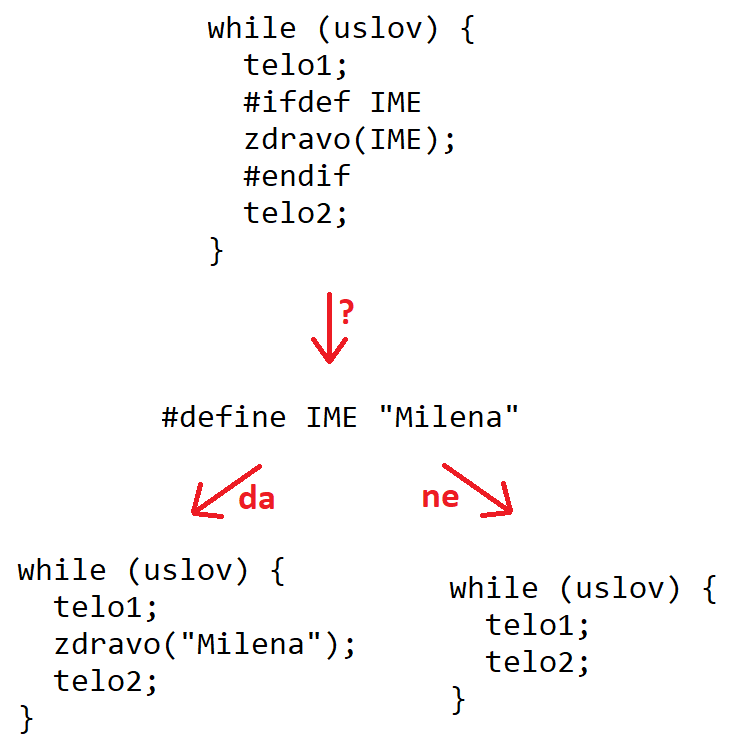
\includegraphics[scale=0.6]{pretproc}
\end{center}
\caption{\dvareda{Двоструки проблем претпроцесирања -- да ли је\\име дефинисано и која му је вредност ако јесте}}
\label{pretproc}
\end{figure}

\section{Закључак}

Кланг се, као део преводилачке инфраструктуре \textit{LLVM}, издваја од конкурената по томе што пружа чист апликативни програмски интерфејс (\textit{API}) према апстрактном синтаксном стаблу (\textit{AST}). Управо тај \textit{API} истражен је у овом раду, на примеру језика \textit{C}, и то конкретно на примеру трансформације петљи у жељени тип. За те потребе написана је апликација која умногоме успешно обавља замишљени посао, инкрементално мењајући текст кода све док не остане само жељени тип петље. У разматрању, као и при самом раду на програму, јавило се неколико углавном ситних проблема. Већина је успешно решена, са главним изузетком када је у питању руковање претпроцесорским директивама, на шта би се могло усмерити даље истраживање.

Такође би се са примећеним ограничењима \textit{API}-ја могло изаћи пред Клангове развијаоце и предложити пригодне измене, односно побољшања, посебно када се узме у обзир да је познато да су ажурни и да радо прихватају корисничке сугестије. Штавише, чињеница је да је у раду коришћена мало старија шеста верзија из марта 2018, док је у актуелној десетој из марта 2020. интерфејс већ измењен, па је тако сад нпр. могуће проверити да ли уведено име гази неко већ постојеће.

\newpage
\addcontentsline{toc}{section}{Литература}
\appendix
\bibliography{Clang-petlje}
\bibliographystyle{unsrt}

\end{document}
